\chapter{Peering Infrastructures}\label{cap:background}
\thispagestyle{empty}

	%In this chapter, we present some background related to the area of the proposed plan. In Section~\ref{sec:peering-infra}, we describe the concepts of Peering Infrastructures, defining Internet Exchange Points (Subsection~\ref{subsec:ixp}) and Colocation Facilities (Subsection~\ref{subsec:colos}).

	%\section{Peering Infrastructures}
	%\label{sec:peering-infra}

	Peering infrastructures are comprised of both Internet exchange points (IXP) and colocation facilities. They are responsible for exchanging a growing volume of traffic between different networks, support thousands of network members, and are widely available all over the world.

	%The studies mentioned below show that these infrastructures are worldwide available and have a comprehensive view of the Internet. Thus, they present an potential opportunity for generating rich geolocation inferences and improve knowledge about the Internet topology.

	\section{Internet Exchange Points}
	\label{subsec:ixp}

	Internet Exchange Points are physical network infrastructures where a set of autonomous systems can interconnect their networks to exchange traffic. Figure~\ref{fig:ixp-topology} shows a typical IXP architecture. IXPs provide a shared switching fabric where participating networks can interconnect their routers. The switch fabric carries the traffic resulting from public and private peering of all interconnected ASes. Each IXP provides one or more \emph{core switches} in the shared fabric for redundancy. They also associate with several Colocation Facilities and install \emph{access switches} to reach city-level interconnection with other networks~\cite{Giotsas:2015:MPI:2716281.2836122}.

	\begin{figure}[t]
	    \centering
	    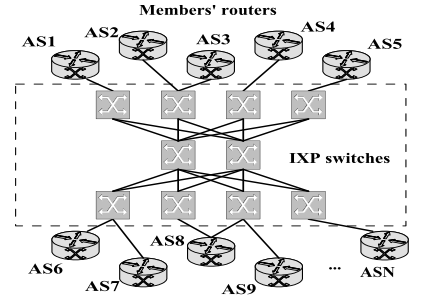
\includegraphics[width=0.5\textwidth]{ixp-topology.png}
	    \caption{A typical IXP architecture~\cite{Ager:2012}}
	    \label{fig:ixp-topology}
	\end{figure}

	Historically, IXPs can be considered as the successors of Network Access Points (NAPs), which were responsible for the smooth transition from the monolithic government network to the modern Internet~\cite{Chatzis:2013}. Since 1995, the four existing NAPs have been replaced by more than 850 IXPs in 200+ cities around the world, interconnecting 50k+ networks~\cite{internetexchangemap, Ager:2012, Giotsas:2015:MPI:2716281.2836122}.

	Studies reveal that existing Internet Exchange Points are responsible for transferring amounts of data similar to Tier 1 Internet Service Provider (ISPs)~\cite{Ager:2012}. Chatzis et al. ~\cite{Chatzis:2013:BUL:2504730.2504746} report that one of the largest European IXPs can observe traffic from a large portion of the Internet, including 42K+ routed ASes, almost all 450K+ routed prefixes and around a quarter billion IP addresses from all the countries around the globe. 

	Richter et al.~\cite{Richter:2014} point a growth of 10-20\% annually in the membership rates of ASes connecting in IXPs of 50-100\% per year in traffic rates. Kotronis et al.~\cite{Kotronis:2015:IPI:2745844.2745877} show that about 40\% of IP prefixes advertised on the Internet can be reached directly from around 5 IXPs. Besides, despite the focus to deploy peering infrastructures in Europe and USA~\cite{Chatzis:2013, Chatzis:2015:QVO:2717646.2717650}, studies reveal that developing regions as Latin America, and Africa are recently increasing the adoption of IXPs to enhance network performance~\cite{DissectingBrazilianIXP, Fanou:2017:ICC:3131365.3131394}.

	%\cite{Chatzis:2013, Chatzis:2015:QVO:2717646.2717650, IXPInternetSociety}

	\section{Colocations Facilities}
	\label{subsec:colos}

	Colocation facilities (Colos) are physical locations which provide essential infrastructures like power, space, cooling, physical security, and storage to their associated autonomous systems. More specifically, it is a place where operators of multiple networks place their networking equipment for interconnection~\cite{BITAG}. The provided amenities lower the infrastructure costs and drive small and medium providers to house their equipment (storage, server, routers) in the Colos.

	The Colos platform connects the member's network to various IXPs, transit networks, cloud/content providers and other ASes in multiple locations worldwide. In large metropolitan areas, a colocation facility operator may install various facilities in the same city, interconnected, to allow access from ASes present at one facility to networks at another facility in the same region~\cite{Giotsas:2015:MPI:2716281.2836122}. Large carrier-neutral companies such as Equinix and Telehouse are the leading operators of colocation facilities all over the world~\cite{Kotronis:2017:STC:3131365.3131388}. 

	


	